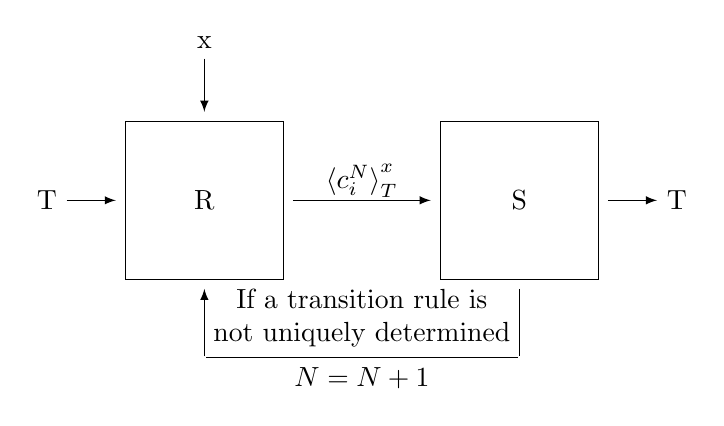
\begin{tikzpicture}

\draw  (-4,3.5) rectangle (-2,1.5);
\draw  (0,3.5) rectangle (2,1.5);
\node (v2) at (-5,2.5) {T};
\node (v1) at (-4,2.5) {};
\node (v4) at (-2,2.5) {};
\node (v3) at (0,2.5) {};
\node (v6) at (2,2.5) {};
\node (v5) at (3,2.5) {T};
\draw [-latex] (v2) edge (v1);
\draw [-latex] (v4) edge (v3);
\draw [-latex] (v6) edge (v5);
\node (v7) at (-3,3.5) {};
\node (v8) at (-3,4.5) {x};
\draw [-latex] (v8) edge (v7);
\node at (-3,2.5) {R};
\node at (1,2.5) {S};
\node at (-1,2.75) {${\langle c_i^N\rangle}_T^x$};
\node at (3,2.5) {};
\node  (v9) at (1,1.5) {};
\node [inner sep=0,outer sep=0](v10) at (1,0.5) {};
\node [inner sep=0,outer sep=0](v11) at (-3,0.5) {};
\node (v12)at (-3,1.5) {};

\draw (v9) edge (v10);
\draw (v10) edge (v11);
\draw  [-latex] (v11) edge (v12);

\node[align=center, below] at (-1,1.5) {If a transition rule is\\not uniquely determined};

\node[below] at (-1,0.5) {$N = N + 1$};
\end{tikzpicture}